\chapter{Data Analysis} \label{DataAnalysis}
This chapter analyzes the results of the 16 users tested. It begins with a validation of findings from past sensorimotor synchronization research and claims mentioned in \ref{SMSfindings}; SMS expectations. 

The results were overall promising, with the haptic modality outperforming audible, as expected, across dynamic beats. Specifically...

\section{Overview}
As previously mentioned, the group was split into 8 Professionals and 4 Non-musicians and 4 Amateurs.\footnote{A special thank you is in order to the professional musicians of the Army Old Guard Fife and Drum Core for volunteering their time.} The level of musical experience varied, as seen in Figure \ref{fig:musicExp}, from less than 1 year to over 10 year. Each user was self-classified as either a Professional, Amateur, or Neither via questionnaire at the end of the test.

\begin{figure}[H]\label{fig:musicExp}
    \centering
    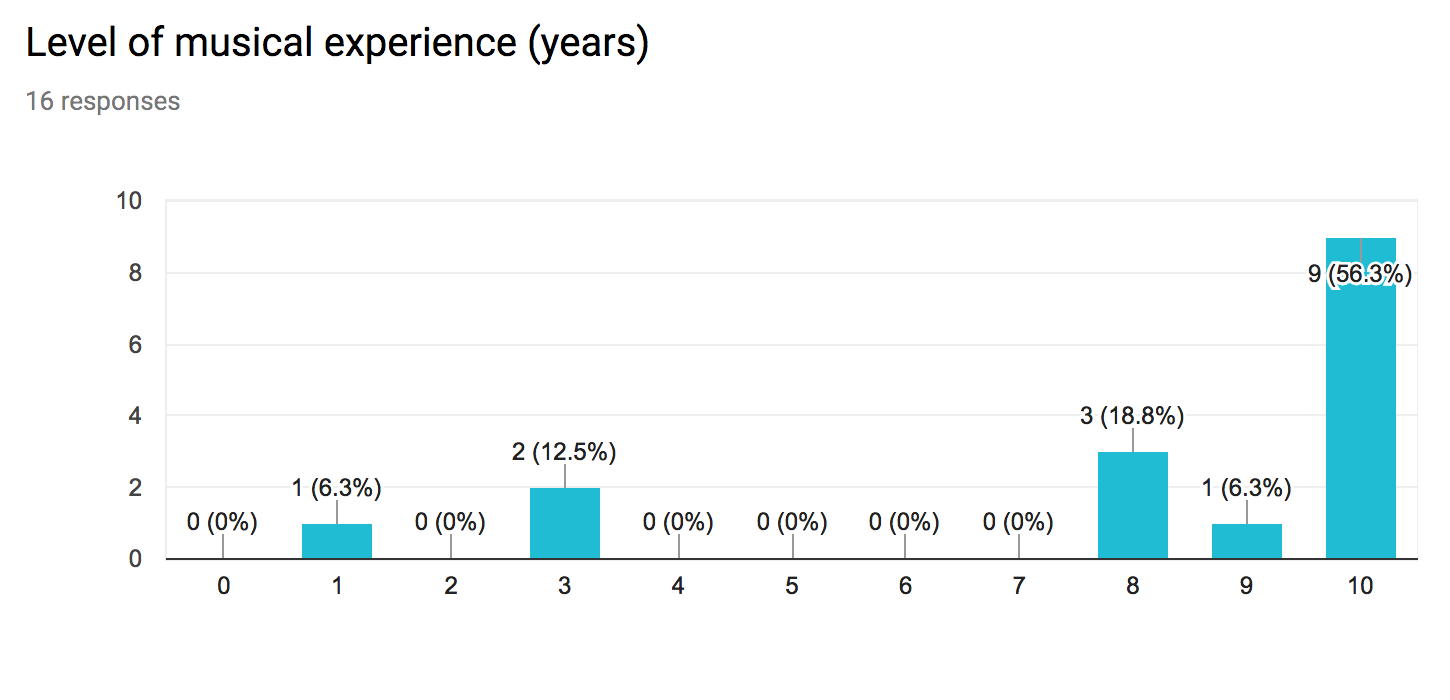
\includegraphics[width=\columnwidth]{musicExp}
    \caption{Musical Experience}
\end{figure}

The instrumental breakdown can be seen in Figure \ref{fig:pieInst}
\begin{figure}[H]\label{fig:pieInst}
    \centering
    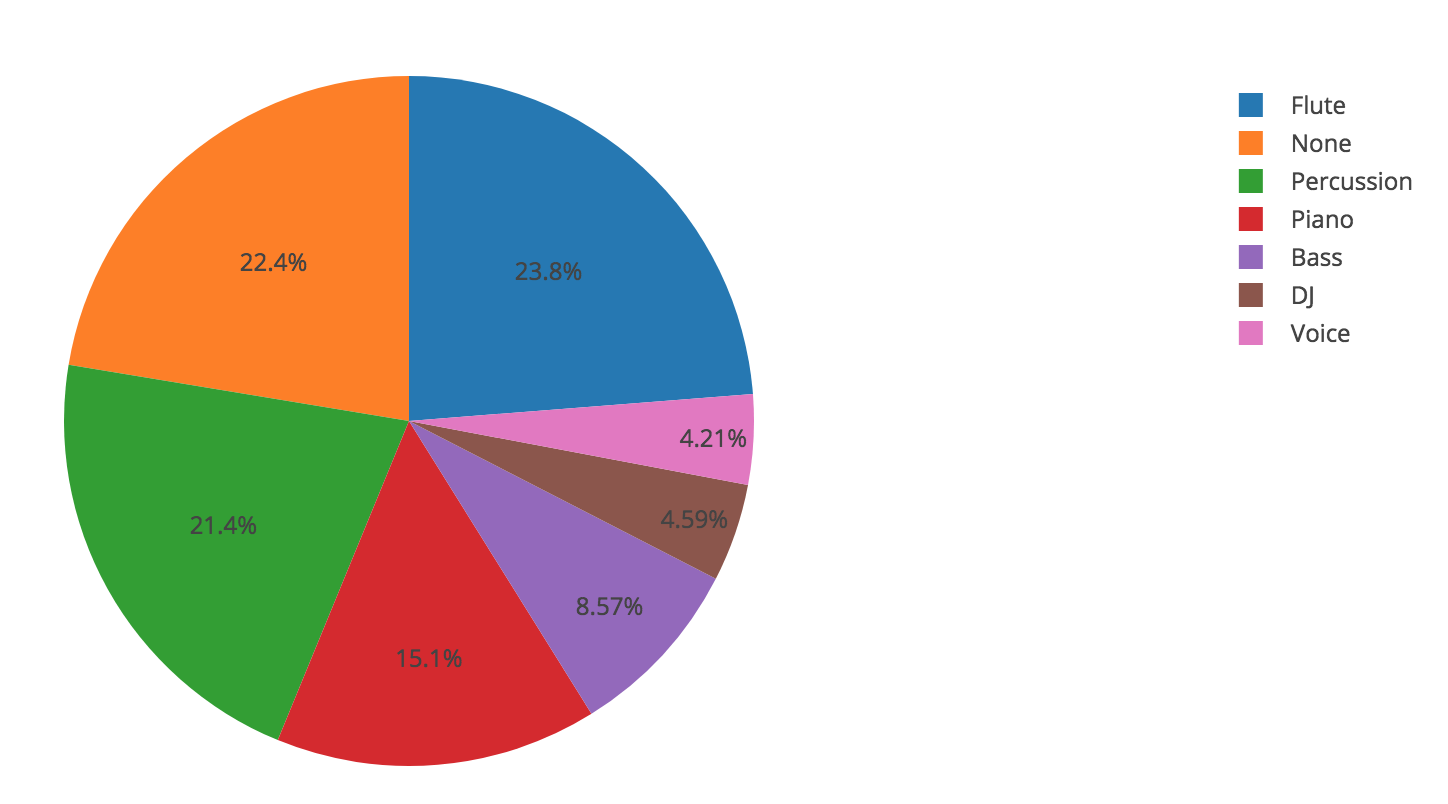
\includegraphics[width=\columnwidth]{pieInst}
    \caption{Spread of instrumental ability (out of 16)}
\end{figure}

Thirteen users had some sort of prior experience with an audible metronome and three did not. For most this was their first experience with a haptic device. All users chose their dominant arm to wear the haptic sleeve and chose their dominant hand to tap with.

\begin{figure}[H]
    \centering
    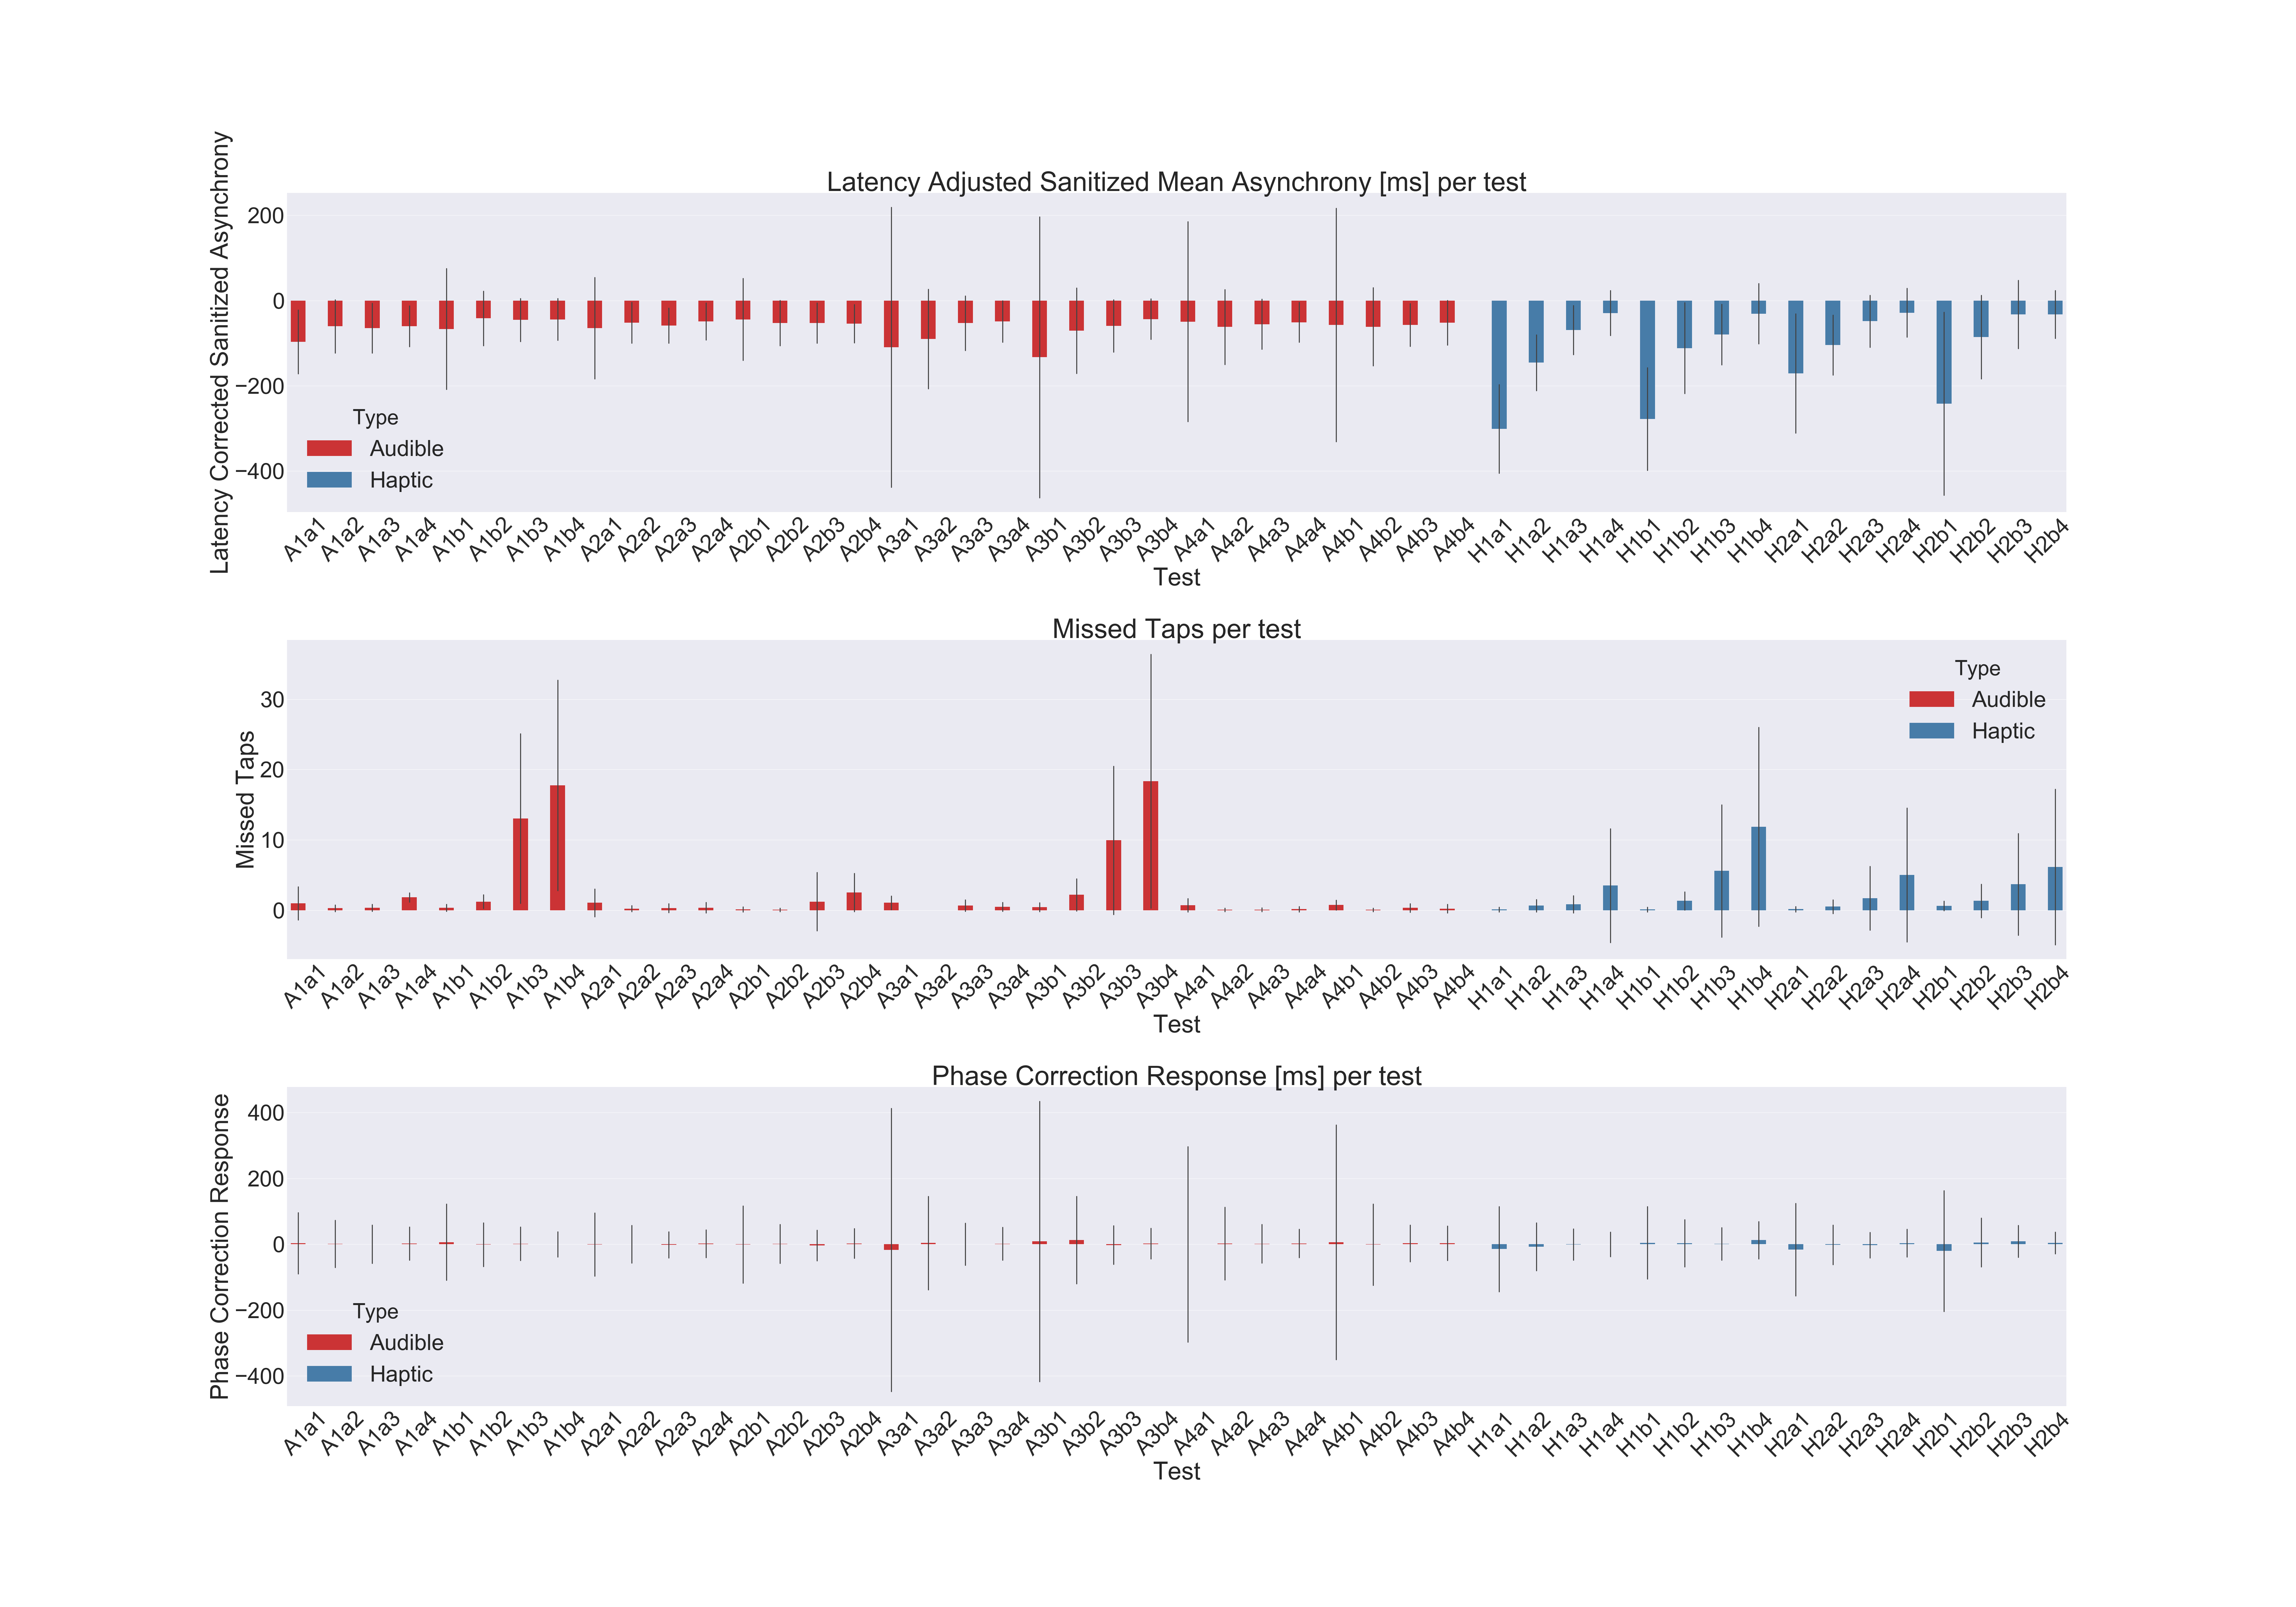
\includegraphics[width=\textwidth]{AllSummary}
    \caption{Summary across all participants}
    \label{fig:AllSummary}
\end{figure}

\begin{figure}[H]
    \centering
    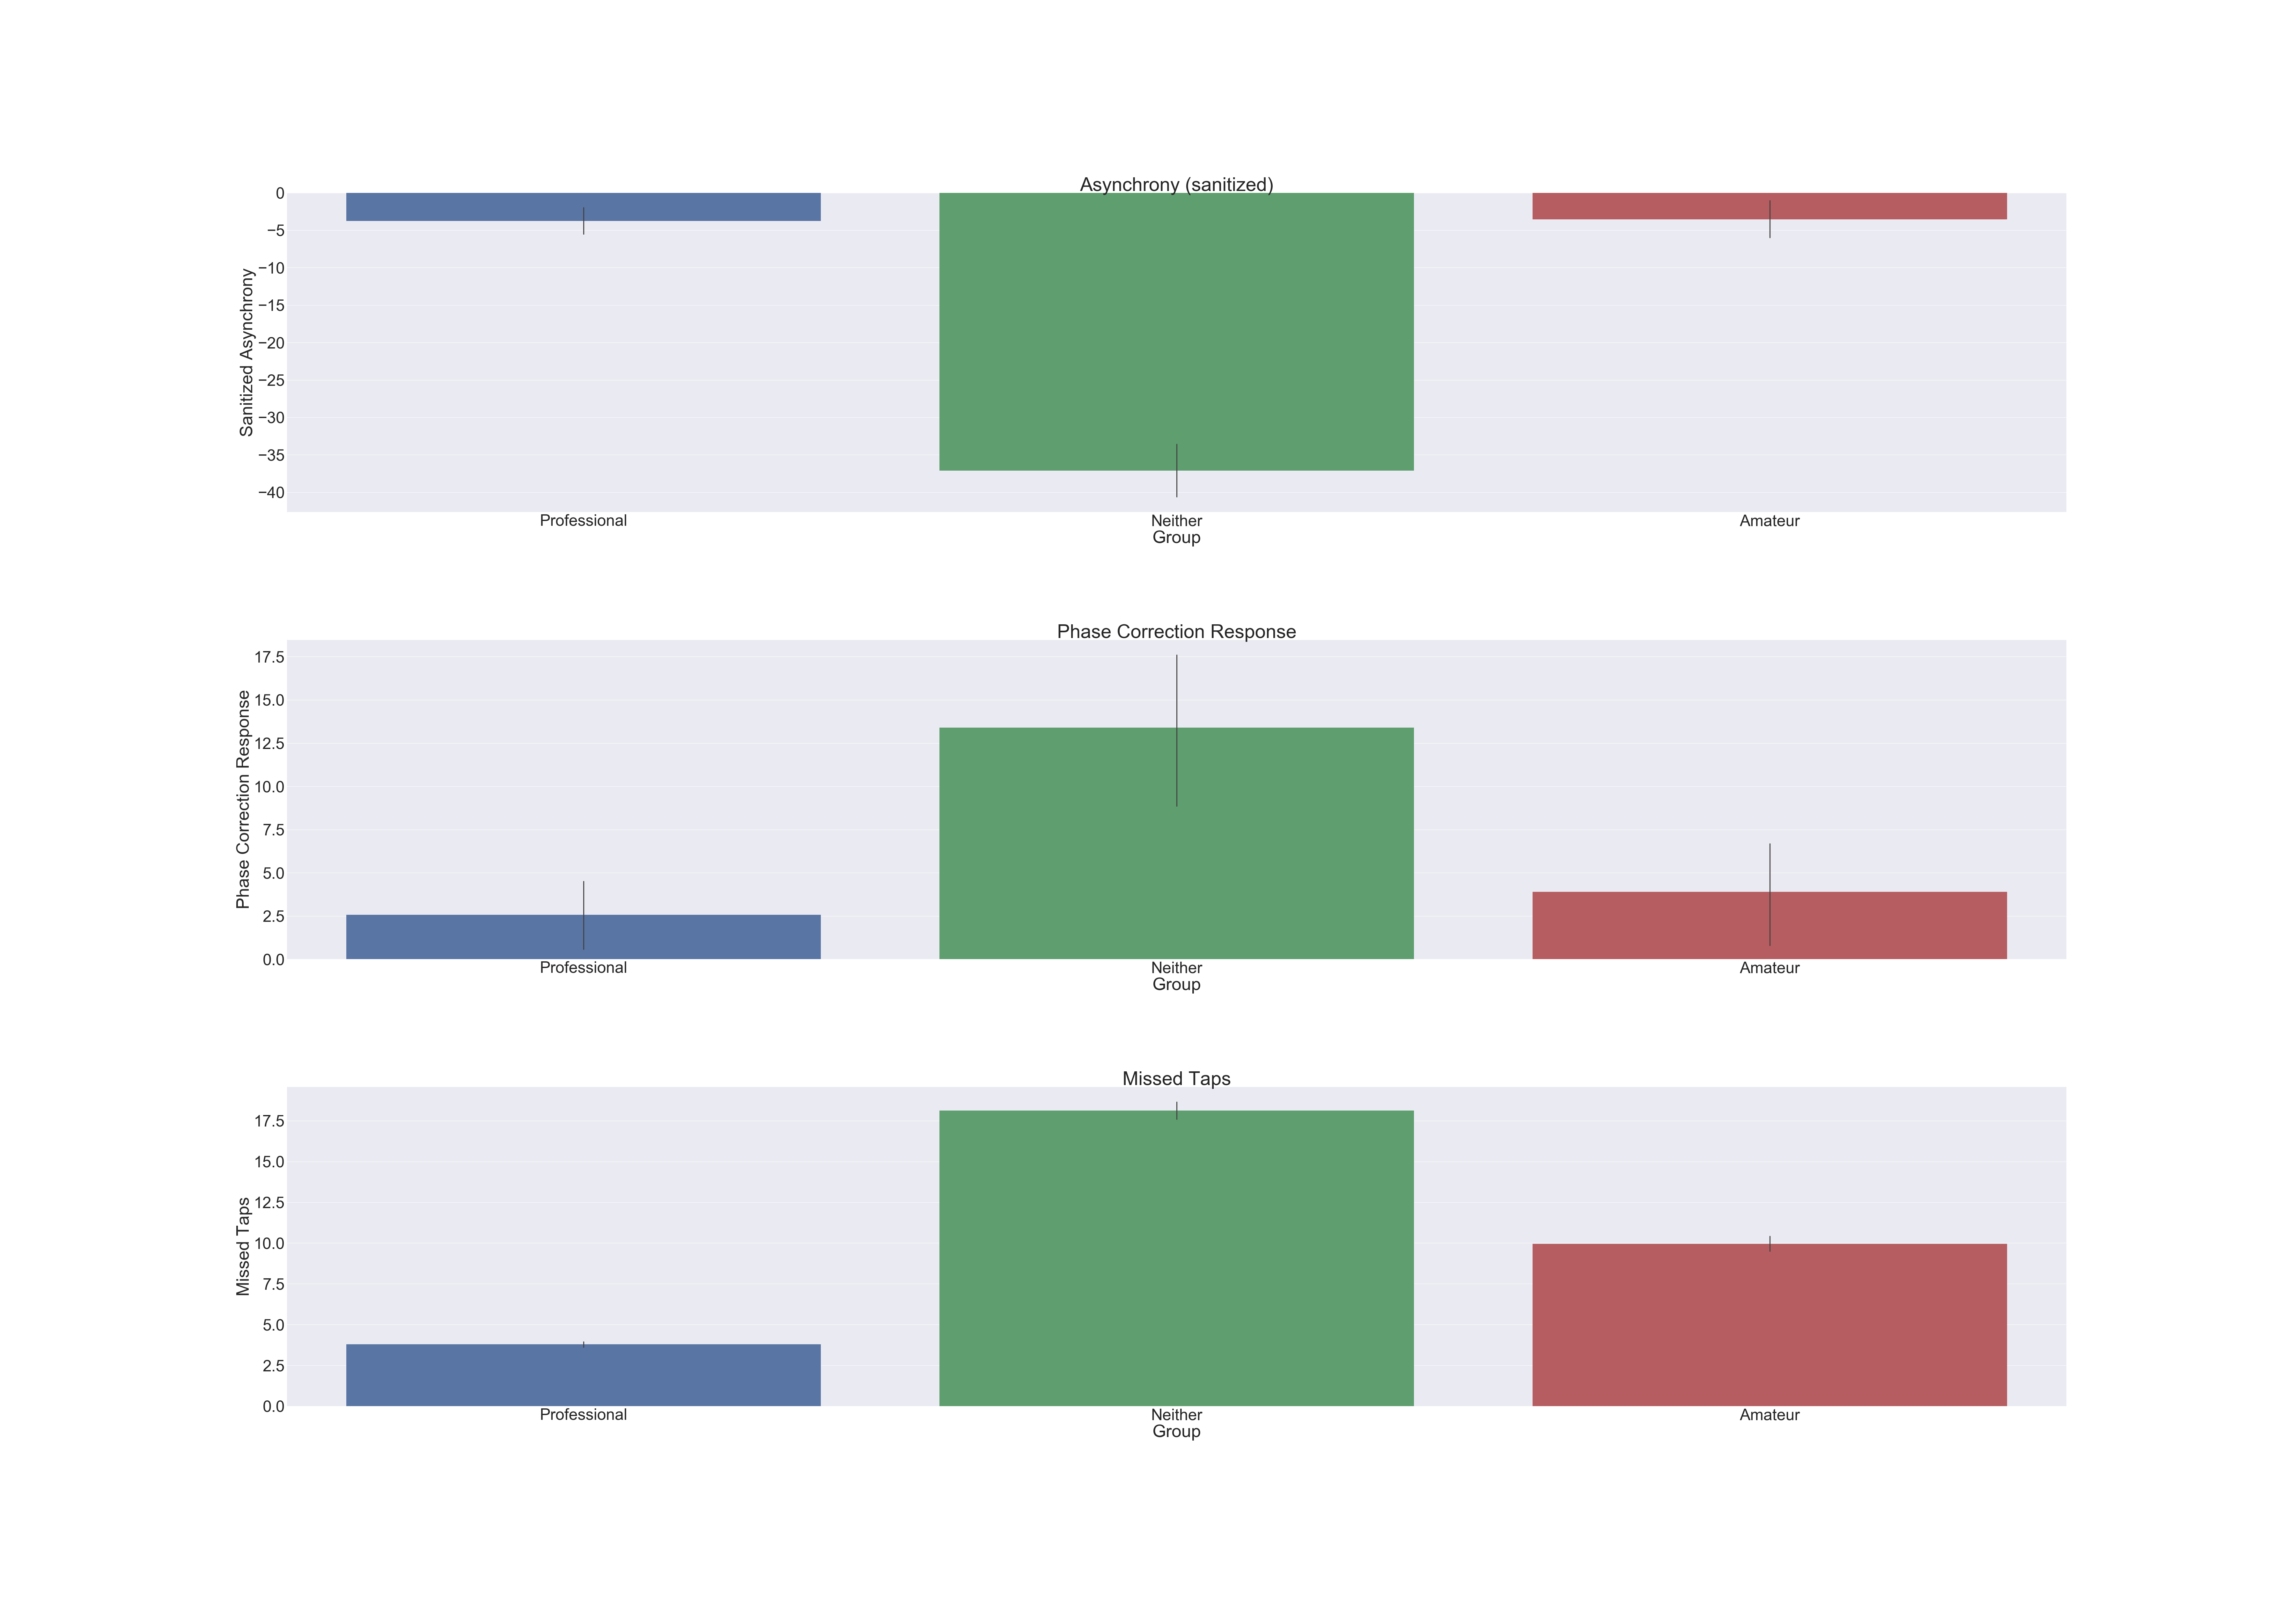
\includegraphics[width=\textwidth]{GroupSummaries}
    \caption{Group test summaries}
    \label{fig:GroupSummaries}
\end{figure}

\begin{figure}[H]
    \centering
    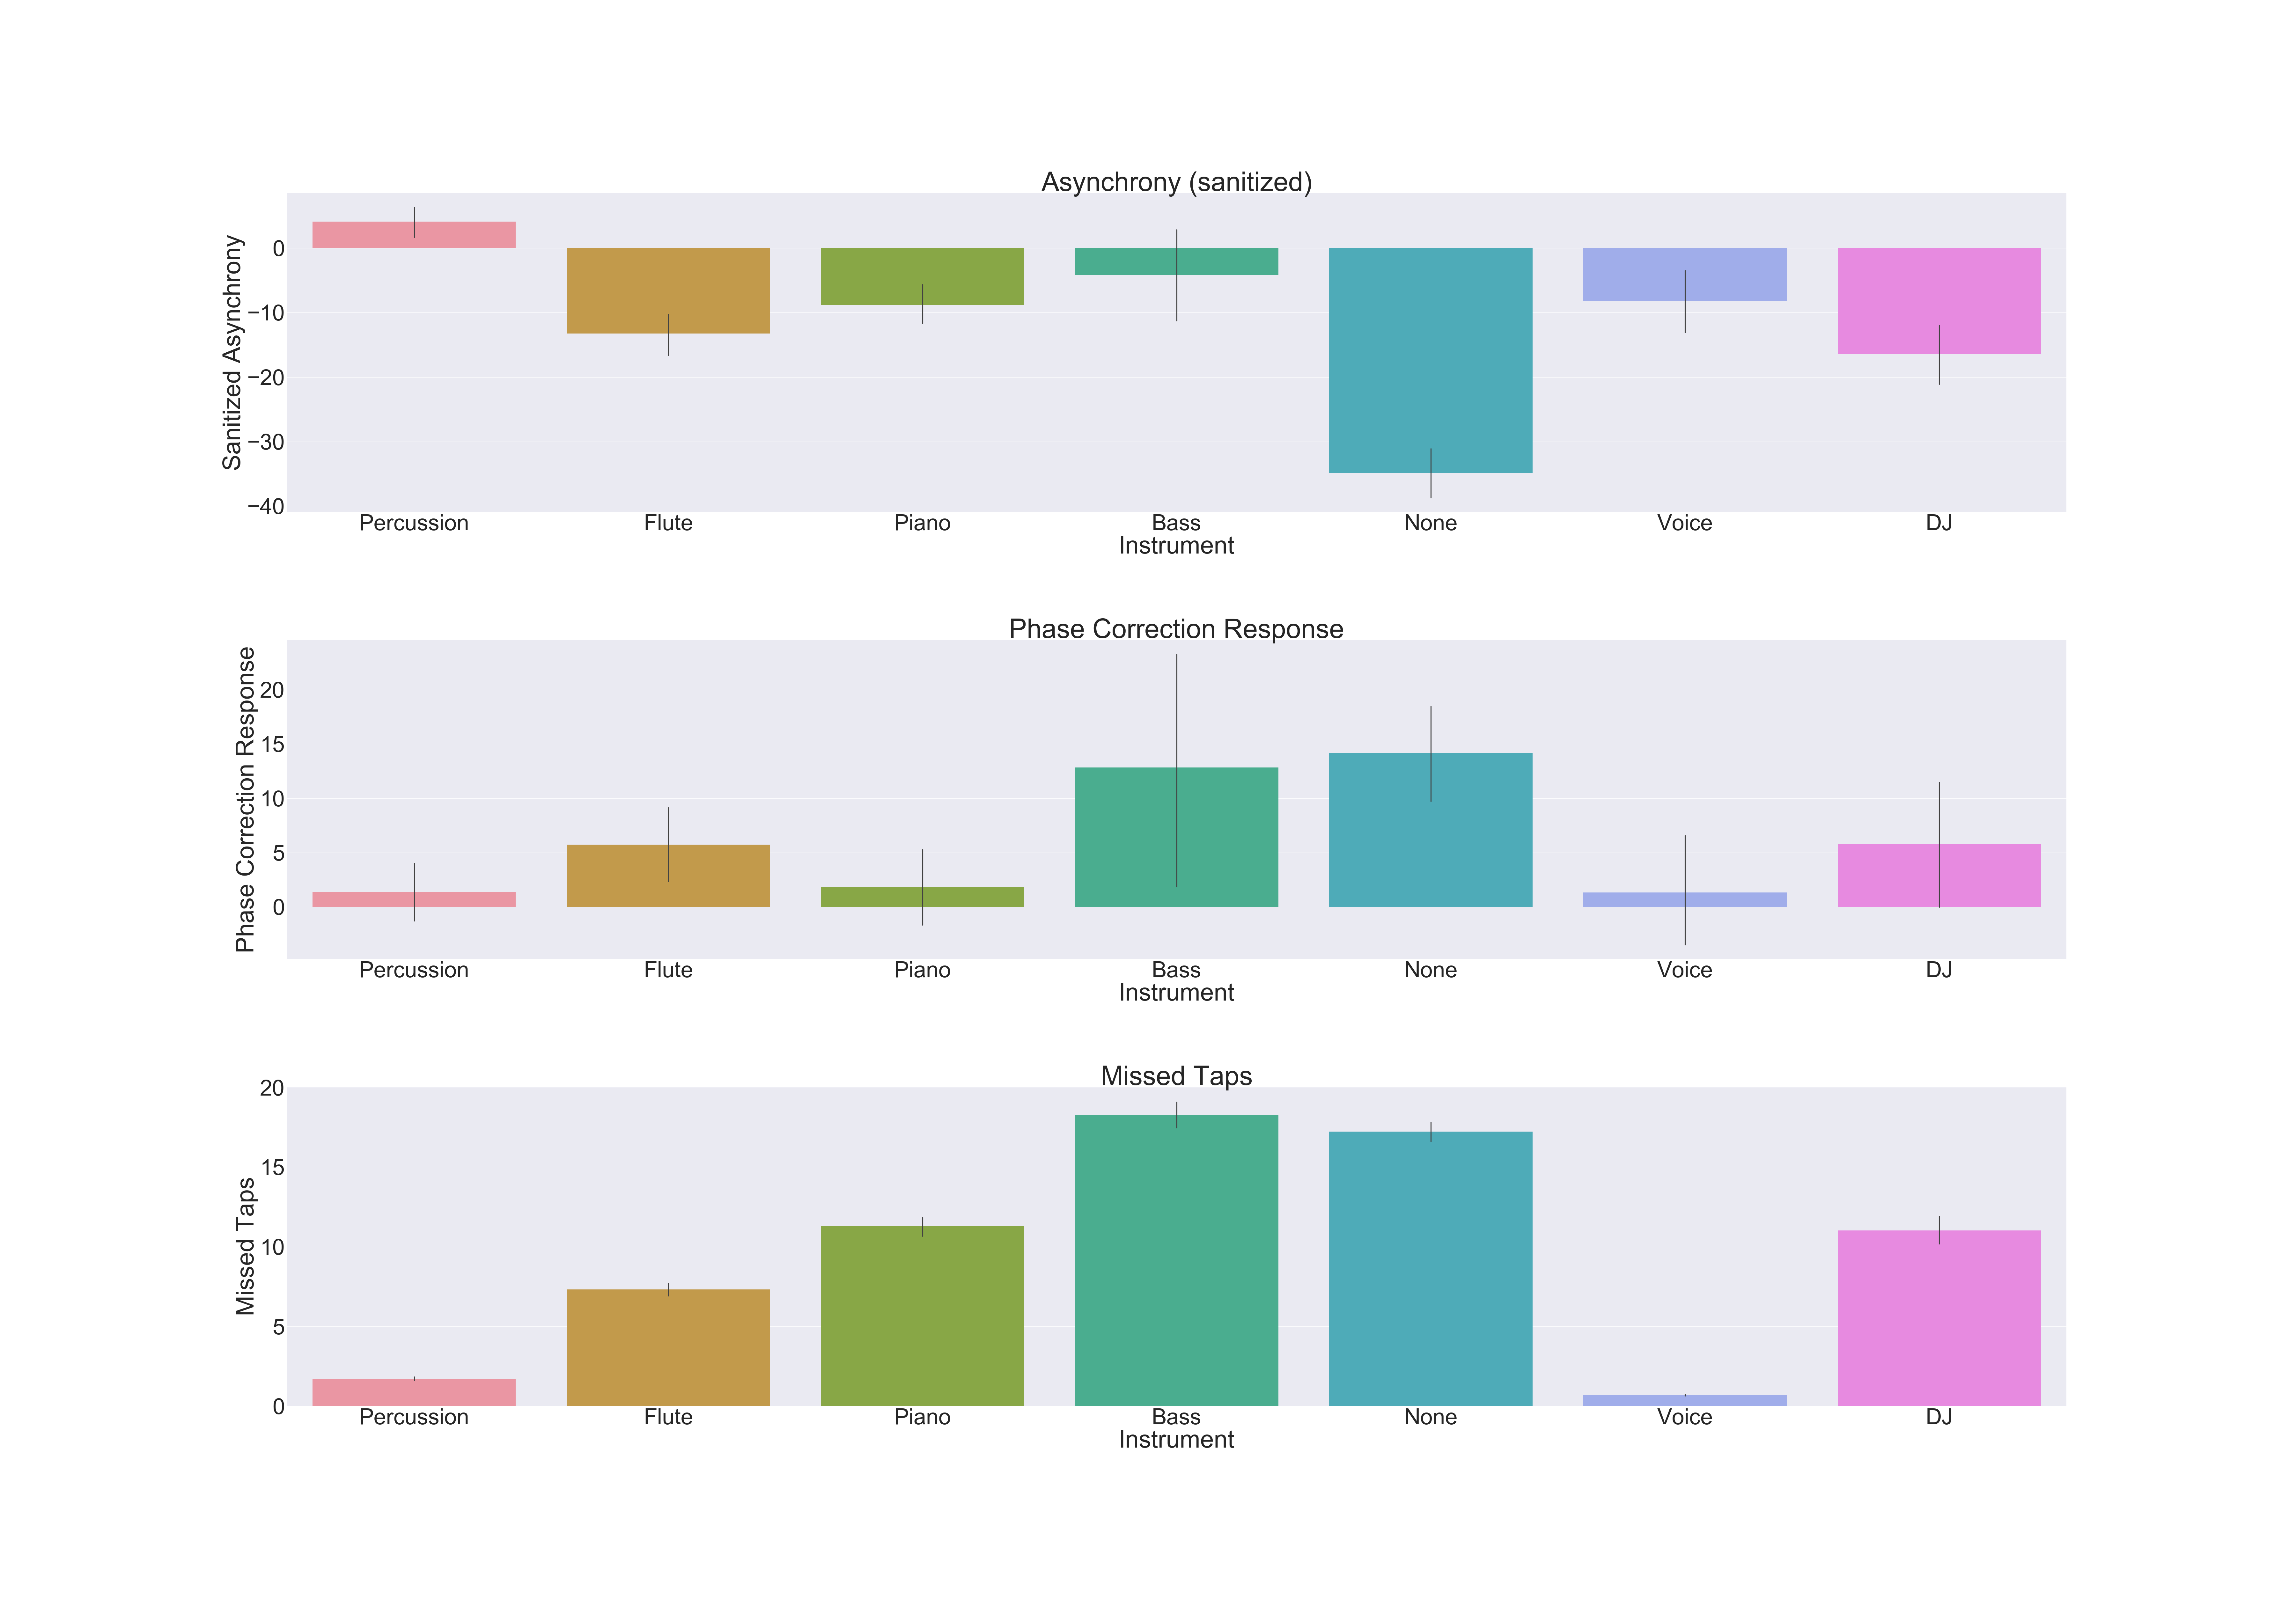
\includegraphics[width=\textwidth]{InstrumentSummaries}
    \caption{Summaries per instrument}
    \label{fig:InstrumentSummaries}
\end{figure}

\section{SMS Research Confirmations}
Expect as IOI increases, $(SD_{asy})$ increases non linearly

Expect linear increase in NMA as IOI increases for non musicians

Expect non-isochronous tapping to introduce distortions within ITI

Expect positive mean asynchrony when approaching biomechanical limit (<300 ms or 180 bpm)

Expect lower $(SD_{asy})$ for professionals vs non musicians

Expect little to no difference between amatuers and non musicians

Expect percussionists and pianists to have the lowest variability

Expect relatively constant NMA for changing IOI (dynamic tests)


\section{Results}

\begin{figure}[H]
    \centering
    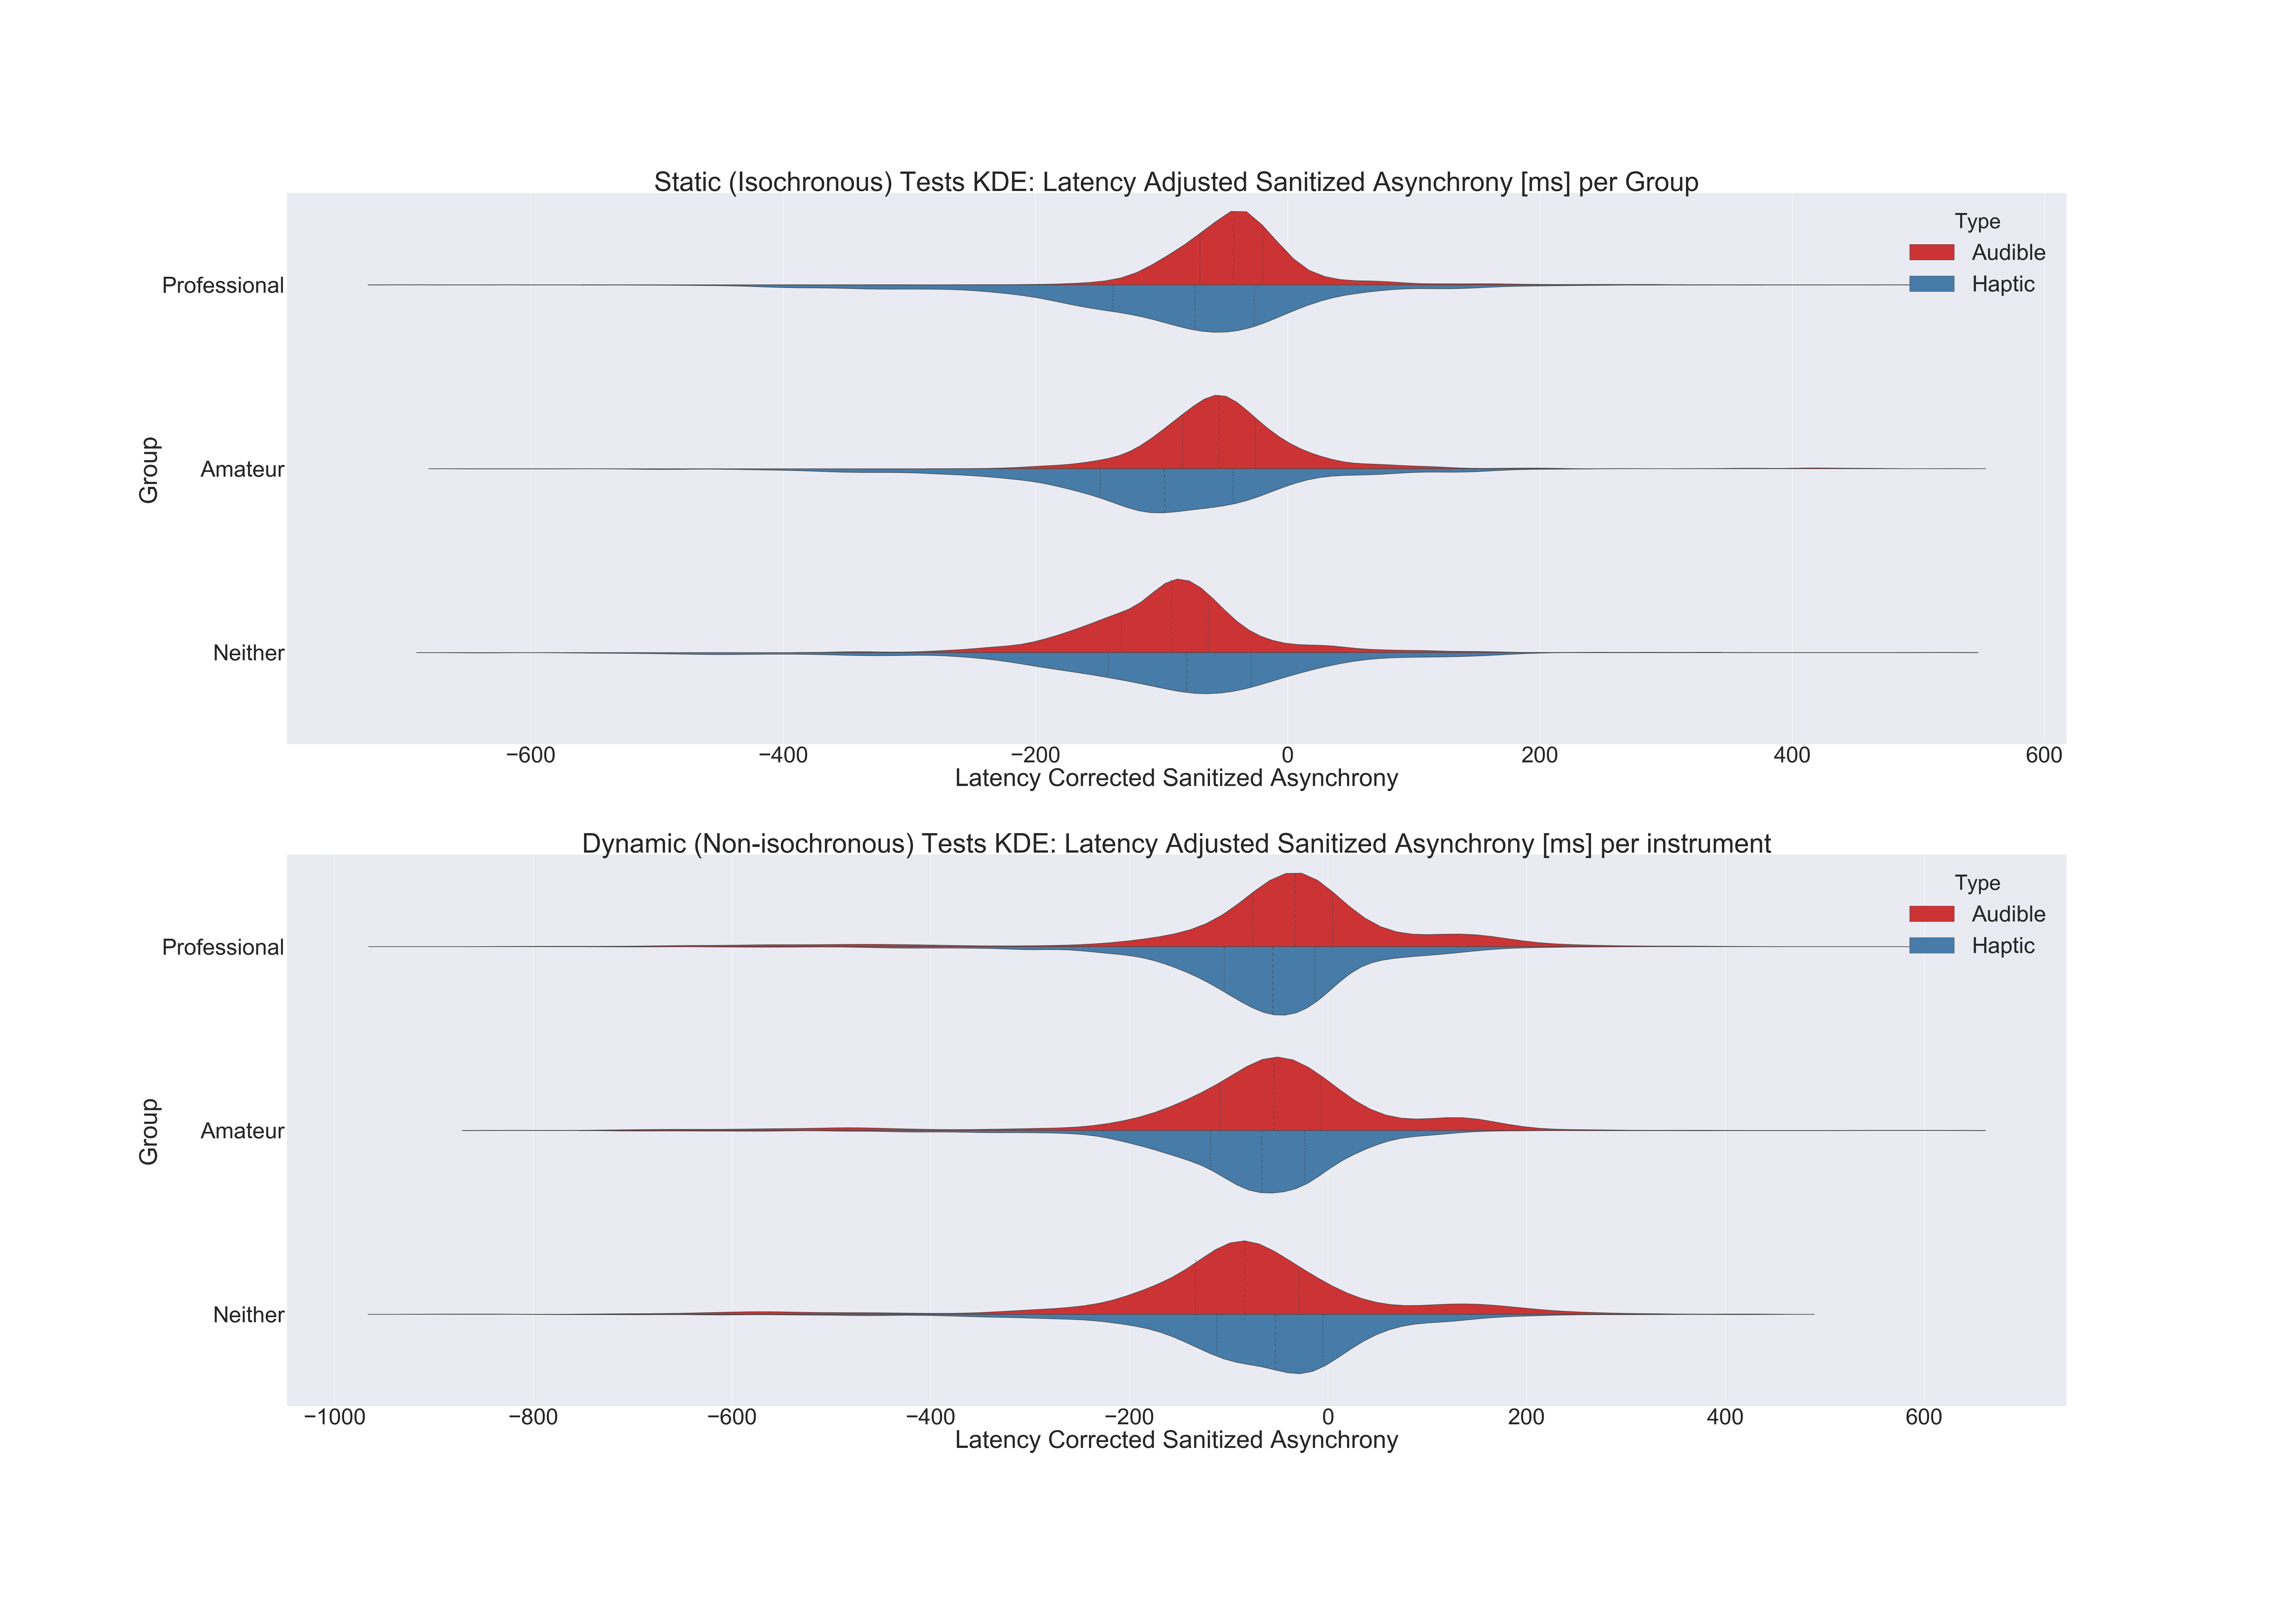
\includegraphics[width=\textwidth]{LCSA_KDE}
    \caption{Kernel Density Estimation: Latency Corrected Sanitized Asynchrony for Static vs Dynamic Tests}
    \label{fig:InstrumentSummaries}
\end{figure}

\begin{figure}[h]
    \centering
    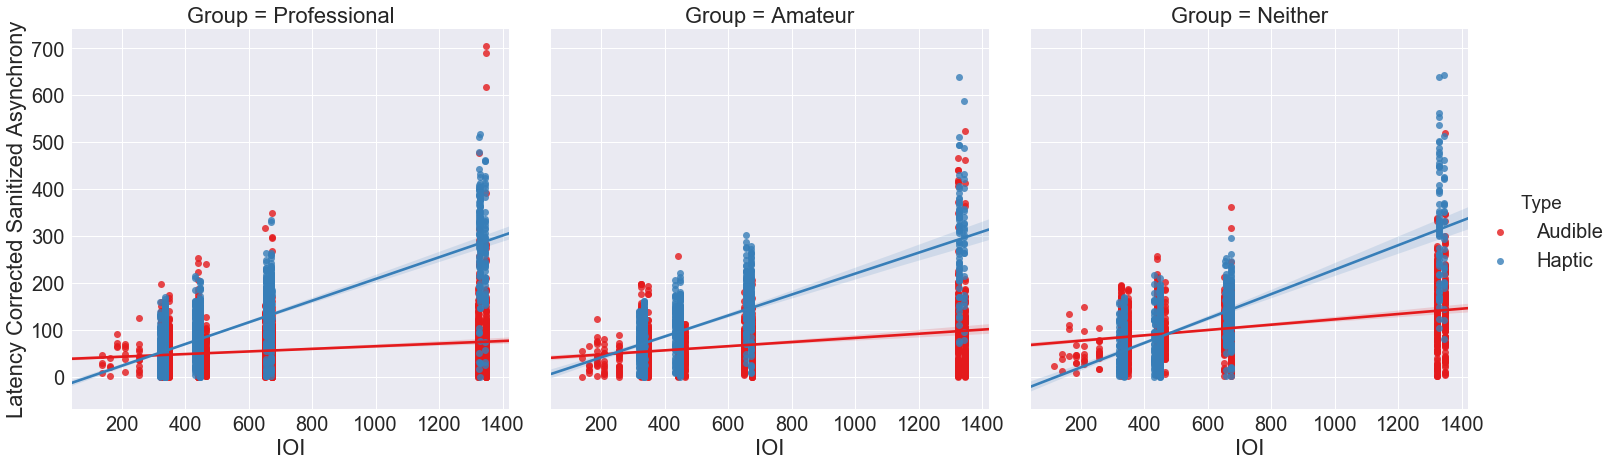
\includegraphics[width=\textwidth]{steady_LCSA_vs_IOI}
    \caption{Latency Corrected Sanitized Asynchrony vs. Inter-Onset-Interval across static test cases.}
    \label{fig:sLCSAvIOI}
\end{figure}

\begin{figure}[H]
    \centering
    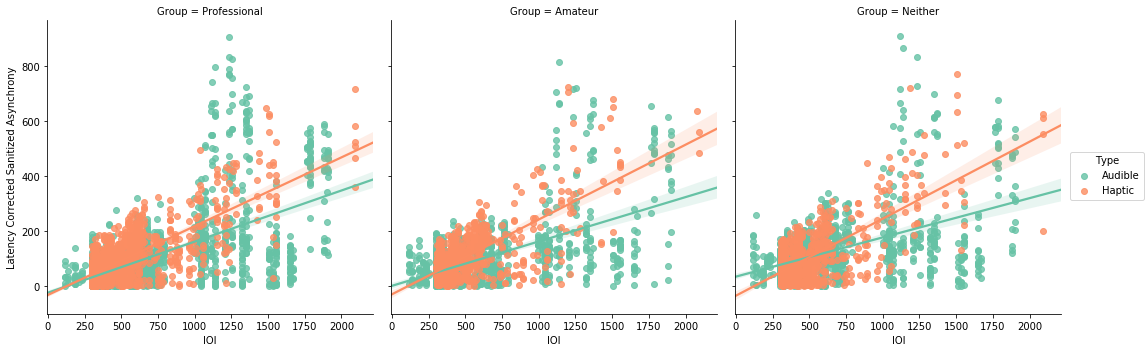
\includegraphics[width=\textwidth]{dynamic_LCSA_vs_IOI}
    \caption{Latency Corrected Sanitized Asynchrony vs. Inter-Onset-Interval across dynamic test cases.}
    \label{fig:dLCSAvIOI}
\end{figure}

\section{Feedback}
On a scale of 1 to 10, with 10 being the most difficult, approximately 70\% of those tested found synchronization to the steady audible beat to be a level of 1, or extremely easy. The remaining 30\% found it to be either a 2 or 4 level of difficulty. However, the spread for dynamic audio test cases was wide ranging with the majority expressing a high level of difficulty 81.3\% above level 5 seen in Figure \ref{fig:Auddiff}.

\begin{figure}[H]
    \centering
    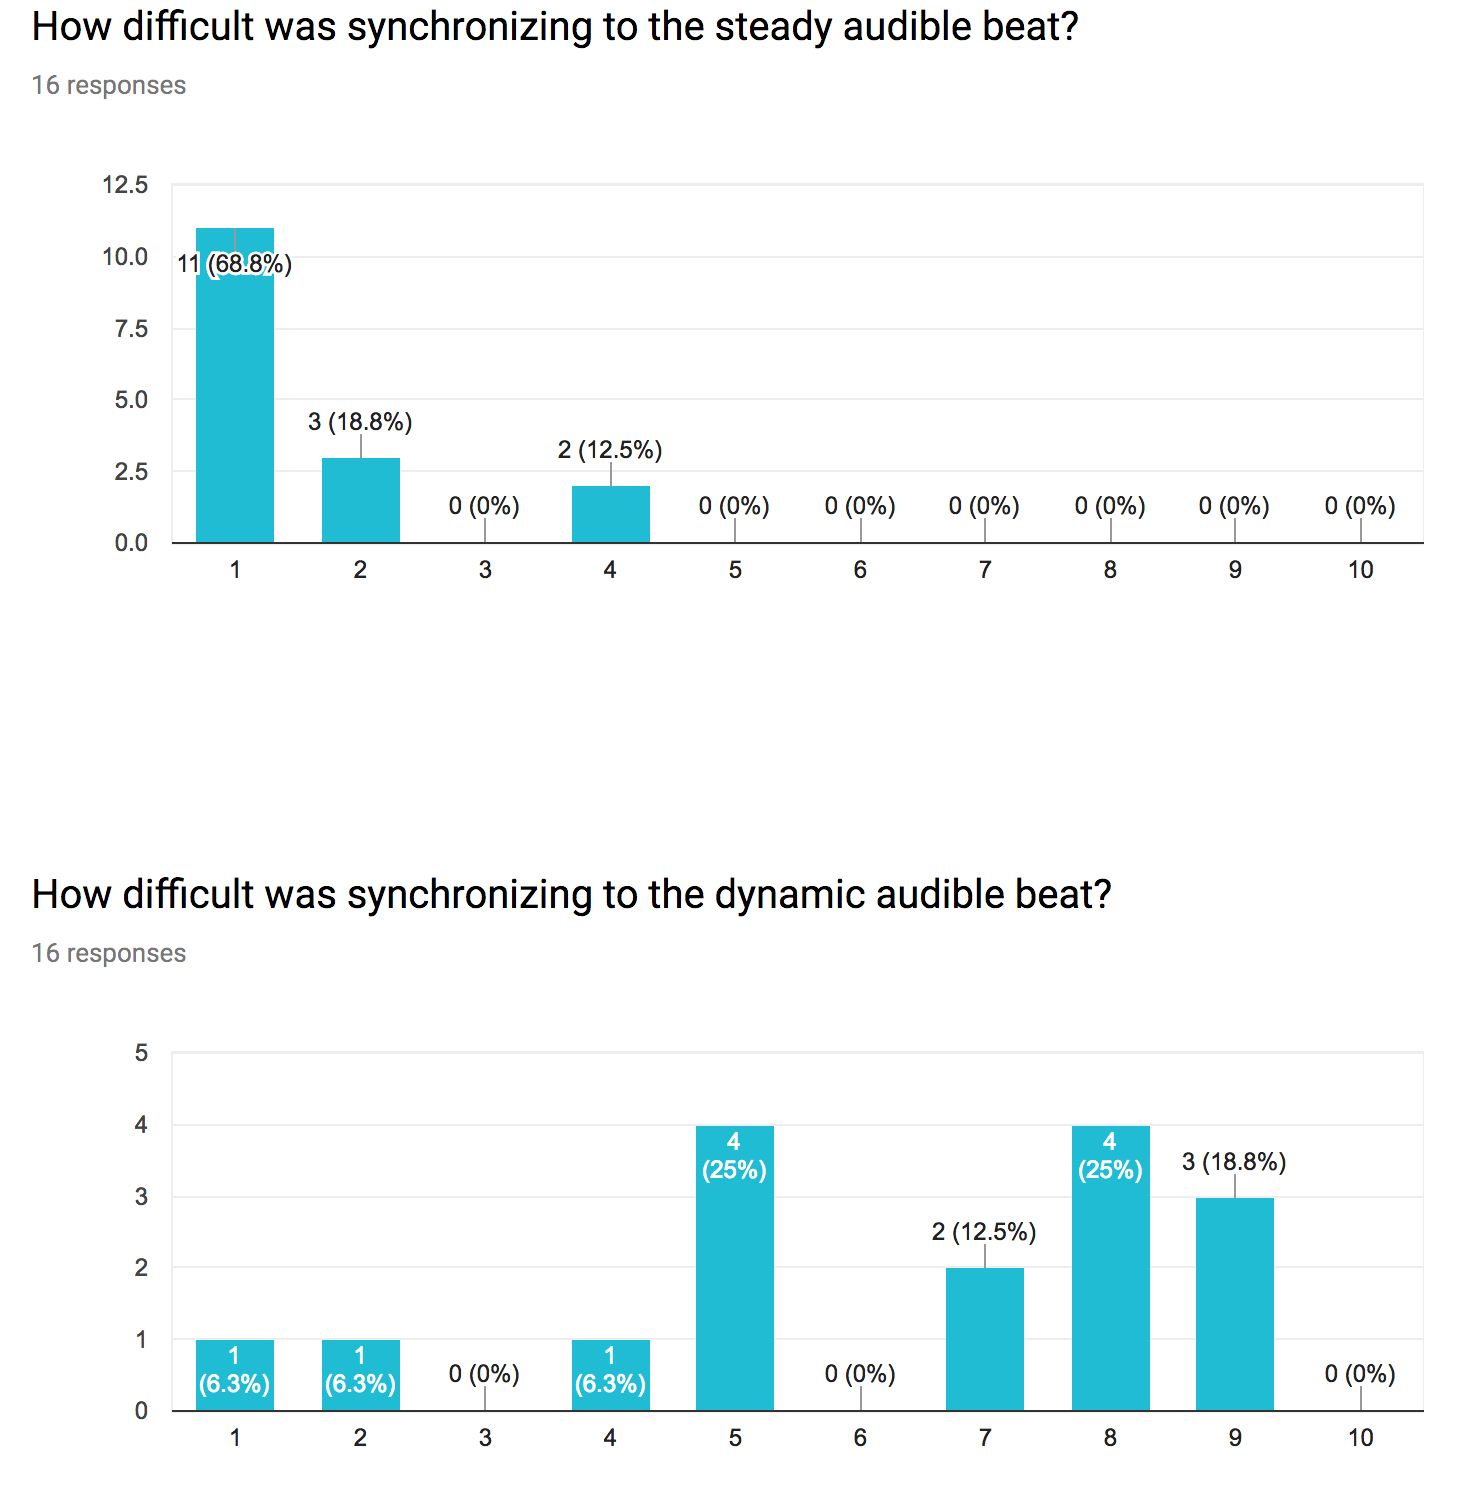
\includegraphics[width=\columnwidth]{Auddiff}
    \caption{Questionnaire: Difficulty results for dynamic audible tests.}
    \label{fig:Auddiff}
\end{figure}

The haptic tests had a wider difficulty spread across the steady beat shown at the top of Figure \ref{fig:Hapdiff}. This was to be expected as users had no prior experience with this haptic device let alone any other sort of wearable metronome. If retested or trained over the course of a few weeks to the sensation of touch the responses might have been more favorable or closer in resemblance to the static audible tests. Regardless, the dynamic beat for the haptic modality yielded less difficulty rankings than the dynamic audible (11 ranked a level of 5 or more difficulty vs. 13 for audible dynamic tests), which further supports the hypothesis of this work.
\begin{figure}[H]
    \centering
    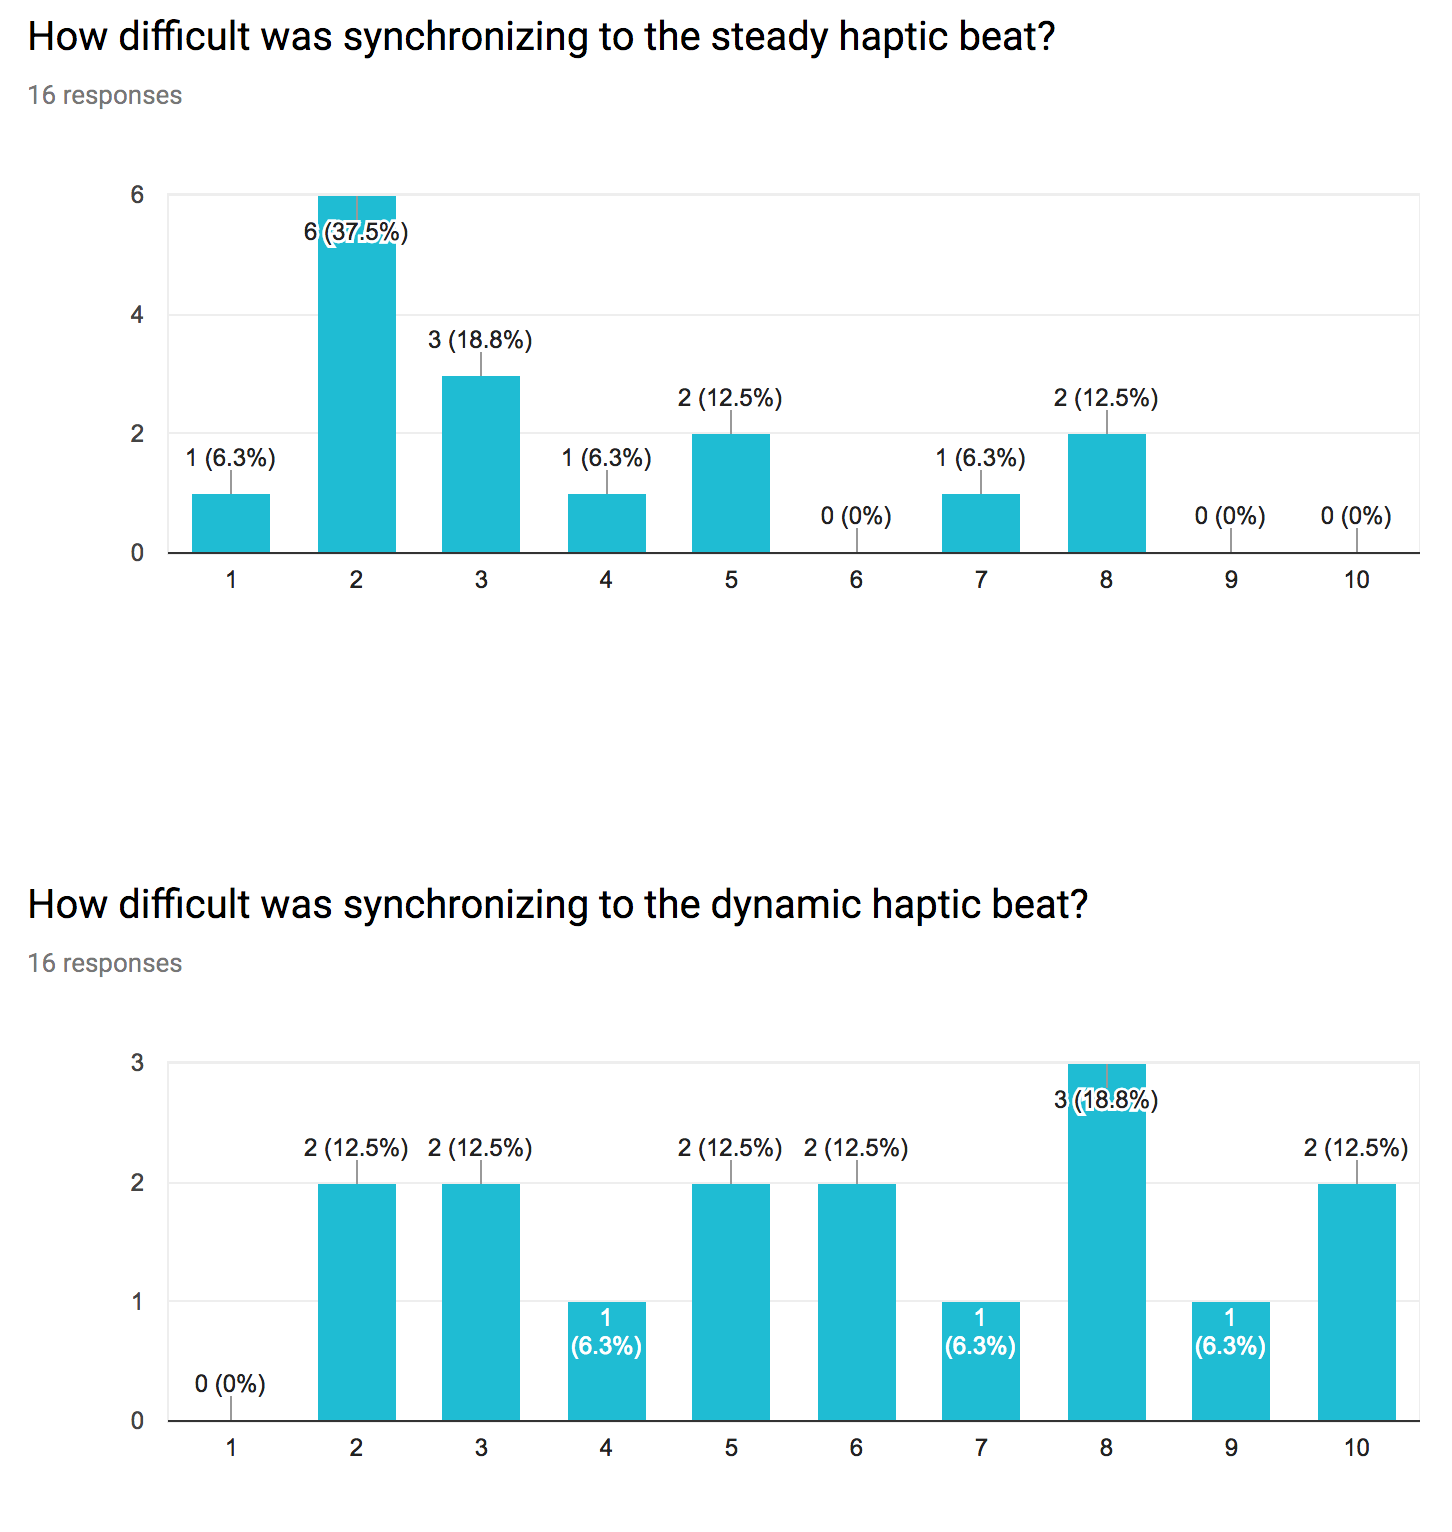
\includegraphics[width=\columnwidth]{Hapdiff}
    \caption{Questionnaire: Difficulty results for dynamic haptic tests.}
    \label{fig:Hapdiff}
\end{figure}

With the question of modality preference, auditory won hands down for the steady beat. Some users would have preferred a combination of both auditory and haptic, though the option was not exemplified throughout in the test suite. The haptic won by 13\% for the dynamic tests, shown in Figure \ref{fig:modPref}
\begin{figure}[H]
    \centering
    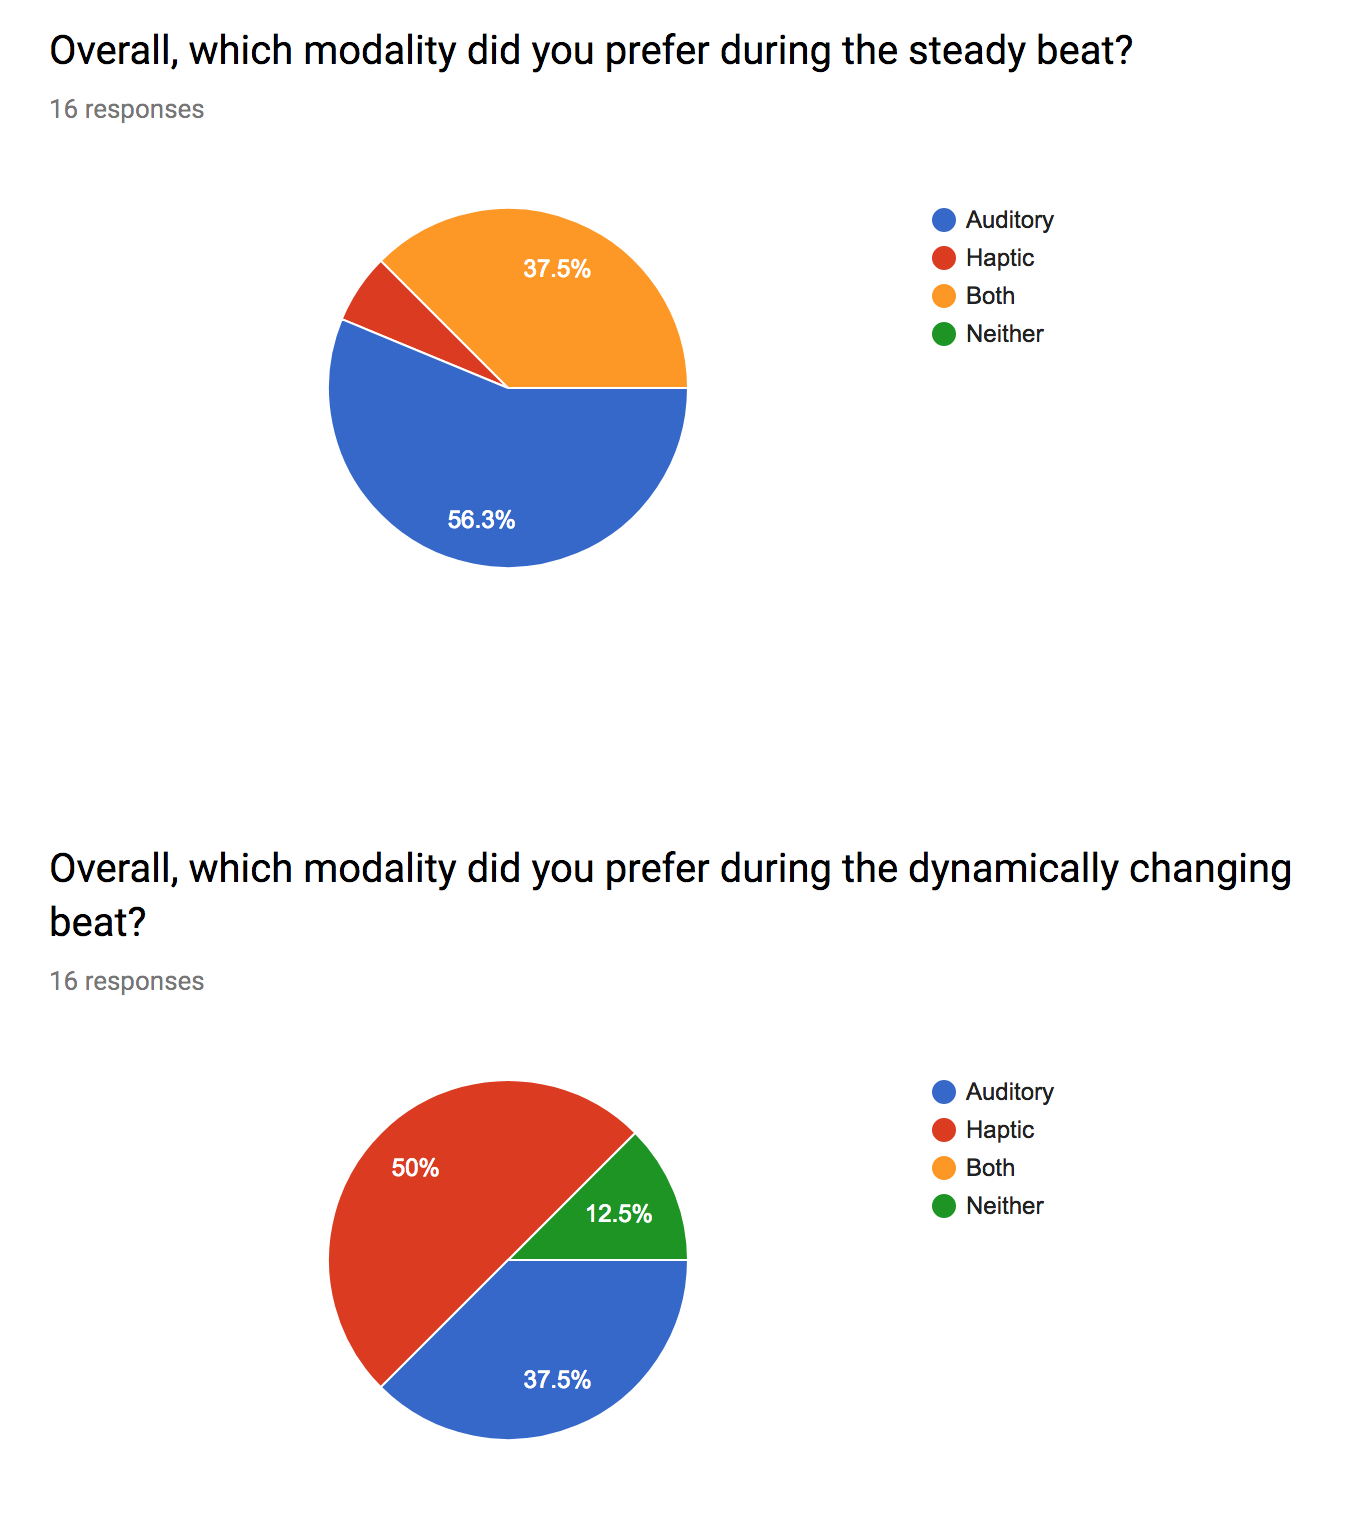
\includegraphics[width=\columnwidth]{modPref}
    \caption{Questionnaire: Modality preference}
    \label{fig:modPref}
\end{figure}

When asked specifically about the preference for haptic mode of operation, it seemed that most users preferred the all on all off mode see in Figure \ref{fig:hspace}
\begin{figure}[H]
    \centering
    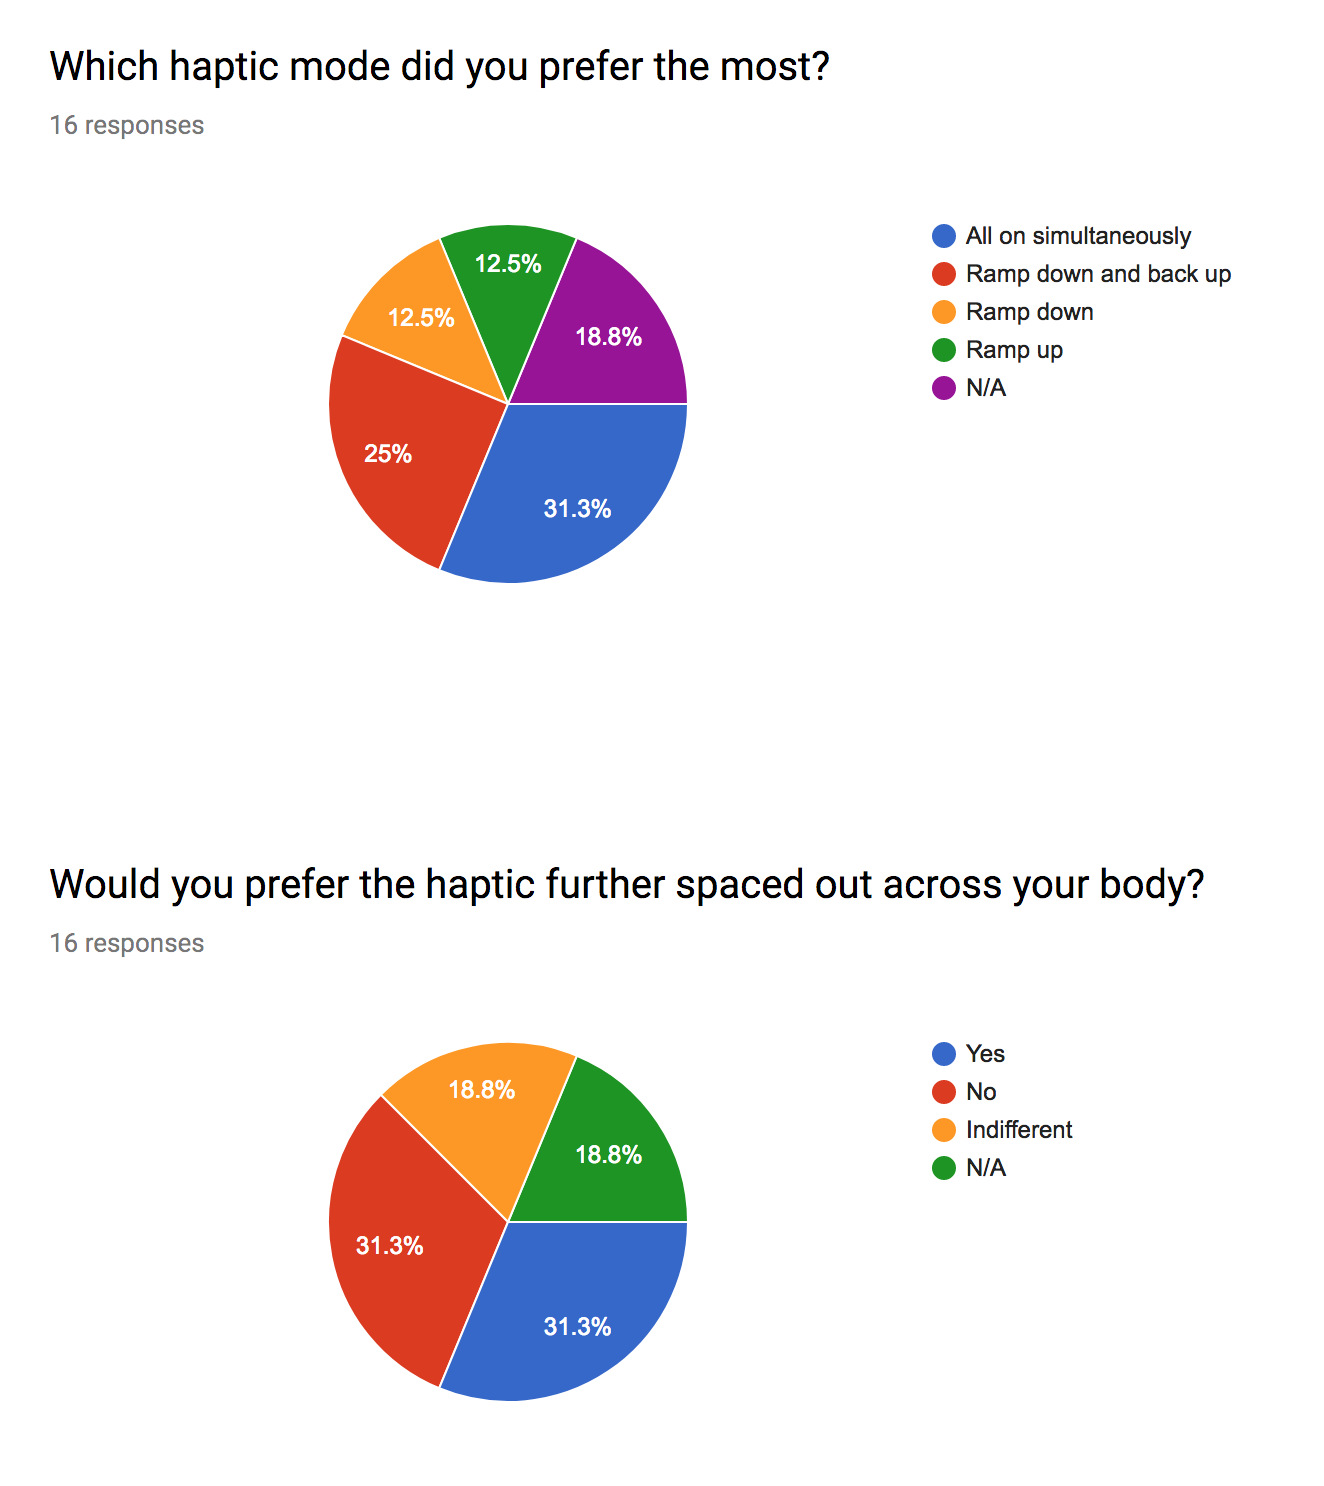
\includegraphics[width=\columnwidth]{hspace}
    \caption{Questionnaire: Haptic mode preference and spacing}
    \label{fig:hspace}
\end{figure}

This could be attributed to the lack of stimulation strength at higher vibrating frequencies for the ramping mode, an intrinsic flaw due to the nature of power operation of the haptic prototype at 5 V 500 mA laptop USB max output - remedied with the battery-dependent next design iteration discussed in Chapter \ref{wirelessHP}. 

Furthermore, the users were tested at up to (and occasionally past) 180. This is well beyond the documented 150 bpm limit. At such rapid speeds the vibrotactiles had little time to ramp up to full capacity. This was another reason for diminished strength and yielded a sensation indistinguishable from noise.

When asked about placement preference, there was a 31.3\% split between the desire to have it further spaced or not. Prior research advocates a larger area of coverage to isolation stimulation zones and therefore promote perceptivity. This would be adopted in a more flexible way on the next prototype iteration with velco straps that can be spaced out however desired.

\section{Conclusions}
